\documentclass[11pt]{article}

\usepackage[margin=1in]{geometry}
\usepackage{amsmath, amssymb}
\usepackage[T1]{fontenc}
\usepackage{lmodern}
\usepackage{microtype}
\usepackage{graphicx}
\usepackage{booktabs}
\usepackage{array}
\usepackage{float}
\usepackage{xcolor}
\usepackage{fancyhdr}
\usepackage[font=small,labelfont=bf,skip=5pt]{caption}

\definecolor{psink}{RGB}{23,54,93}
\definecolor{psaccent}{RGB}{192,80,77}
\definecolor{psrule}{RGB}{200,209,222}

\usepackage[colorlinks=true,allcolors=psink]{hyperref}

\graphicspath{{Part1/}{Part2/figs/}}
\emergencystretch=3em

\setlength{\textfloatsep}{10pt plus 2pt minus 2pt}
\setlength{\intextsep}{10pt plus 2pt minus 2pt}
\setlength{\abovecaptionskip}{4pt}
\setlength{\belowcaptionskip}{0pt}

\makeatletter
\renewcommand\section{\@startsection{section}{1}{0pt}%
  {-2.6ex \@plus -1ex \@minus -.2ex}{1.3ex \@plus .2ex}%
  {\normalfont\bfseries\scshape\large\color{psink}}}
\renewcommand\subsection{\@startsection{subsection}{2}{0pt}%
  {-2.2ex \@plus -1ex \@minus -.2ex}{1.0ex \@plus .2ex}%
  {\normalfont\bfseries\normalsize\color{psink}}}
\renewcommand\subsubsection{\@startsection{subsubsection}{3}{0pt}%
  {-1.9ex \@plus -.8ex \@minus -.2ex}{0.8ex \@plus .2ex}%
  {\normalfont\bfseries\itshape\normalsize\color{psink}}}
\renewcommand\subparagraph{\@startsection{subparagraph}{5}{0pt}%
  {-1.6ex \@plus -.6ex \@minus -.2ex}{0.5ex \@plus .1ex}%
  {\normalfont\itshape\normalsize\color{psink}}}
\renewcommand\paragraph{\@startsection{paragraph}{4}{0pt}%
  {1.7ex \@plus 1ex \@minus .2ex}{-0.9em}%
  {\normalfont\bfseries\normalsize\color{psink}}}
\makeatother

\newenvironment{tight}
  {\begin{itemize}\setlength{\itemsep}{3pt}\setlength{\parskip}{0pt}%
   \setlength{\topsep}{3pt}\setlength{\leftmargini}{1.4em}}
  {\end{itemize}}

\setcounter{secnumdepth}{0}   % headings carry the assignment's own labels
\setlength{\headheight}{14pt}
\pagestyle{fancy}
\fancyhf{}
\fancyhead[L]{\footnotesize\scshape\color{psink} MGT 595 \textemdash\ Problem Set 3}
\fancyhead[R]{\footnotesize\color{psink}\thepage}
\renewcommand{\headrulewidth}{0.4pt}
\renewcommand{\headrule}{\hbox to\headwidth{%
  \color{psrule}\leaders\hrule height \headrulewidth\hfill}}

\begin{document}

\thispagestyle{empty}
\begin{flushleft}
{\bfseries\LARGE\color{psink} Quantitative Investing}\\[3pt]
{\scshape\Large\color{psink} Problem Set 3}\\[10pt]
{\color{psrule}\rule{\textwidth}{1.2pt}}\\[5pt]
{\small Ashley Wen\,(xw564)\quad\textbar\quad Emily Wu\,(esw63)%
\quad\textbar\quad Grace Gu\,(xg325)\hfill \today}
\end{flushleft}

\vspace{1.4em}

{\color{psink}\textbf{Contents.}} Part I tests the CAPM on the 49
value-weighted industry portfolios. Part III contains the three standalone AI
exercises and the capstone, a cross-sectional test of U.S.\ sector ETFs. Part
II repeats the tests on the 25 size and book-to-market portfolios and examines
Roll's critique using in-sample and out-of-sample tangency portfolios.

\vspace{0.8em}


% =====================================================================
\section{Part I: 49 Industry Portfolios}
% =====================================================================

\paragraph{Data and conventions.} All figures are in percent per month.
Observations coded $-99.99$ or $-999$ are treated as missing. Industry returns
are total returns, while the market proxy is reported as $R_M - R_f$. We
therefore subtract the monthly riskless rate from each industry return and
work in excess returns throughout. Six industries have no data before the late
1960s, so all 49 series are populated only from July 1969. We report the
balanced July 1969 -- June 2026 panel ($T = 684$, $N = 49$) as our primary
specification. The full July 1926 -- June 2026 sample ($T = 1200$, $N$ from 40
to 49) is reported as a robustness check. The sample mean of $R_M - R_f$ is
$0.6116$ on the balanced sample and $0.6952$ on the full sample.

\subsection{Question (a)}

In the cross-sectional regression
$R_i = \gamma_0 + \gamma_M \beta_{iM} + \eta_i$ with
$\beta_{iM} = \mathrm{cov}(R_i, R_M)/\sigma^2(R_M)$, each observation is a
portfolio, so $\gamma_0$ is the expected return on a portfolio with zero market
beta and $\gamma_M$ is the expected return per unit of beta.

\paragraph{Sharpe\slash Lintner.} With unrestricted borrowing and lending at
the riskless rate, $E[R_i] = R_f + \beta_{iM}(E[R_M] - R_f)$, so
\[
\gamma_0 = R_f, \qquad \gamma_M = E[R_M] - R_f .
\]
Both are exact point predictions. A portfolio with $\beta_{iM} = 0$ bears no
systematic risk and must earn the riskless rate, which fixes the intercept. The
market has $\beta_{iM} = 1$, so the line must pass through $(1, E[R_M])$, which
fixes the slope at the market risk premium.

\paragraph{Black.} Without riskless borrowing and lending, $R_f$ is replaced by
the expected return on the zero-beta portfolio $R_z$, the minimum-variance
portfolio uncorrelated with the market, giving
$E[R_i] = E[R_z] + \beta_{iM}(E[R_M] - E[R_z])$ and
\[
\gamma_0 = E[R_z], \qquad \gamma_M = E[R_M] - E[R_z] .
\]
Because $E[R_z]$ is not observable, this version predicts no specific
intercept. It restricts only $\gamma_M > 0$ and $\gamma_0 < E[R_M]$, and is
therefore weaker and harder to reject: Sharpe\slash Lintner is Black plus the
restriction $E[R_z] = R_f$. Both imply $\gamma_0 + \gamma_M = E[R_M]$, so they
differ only in where the security market line is anchored.

Because all tests use excess returns, the Sharpe\slash Lintner null becomes
$\gamma_0 = 0$ with $\gamma_M$ equal to the average market excess return, and
Black predicts $\gamma_0 = E[R_z] - R_f$, unrestricted in sign but generally
positive.

\subsection{Question (b)}

Each industry's beta is estimated once by OLS over the full sample and held
fixed thereafter; the estimates range from $0.516$ (Utilities) to $1.514$
(Software), with mean $1.039$. In each of the 684 months we then estimate
$R_{it} = \gamma_{0t} + \gamma_{Mt} b_{iM} + \eta_{it}$ across the 49
industries. The monthly slopes are highly volatile, with a standard deviation
of $7.13$ against a mean of $0.035$, and are positive in only $48.4\%$ of
months. Finally we average the monthly estimates, using
\[
\hat\gamma_j = \frac{1}{T}\sum_{t=1}^{T}\hat\gamma_{jt},
\qquad
s(\hat\gamma_j) = \frac{\sigma(\hat\gamma_{jt})}{\sqrt{T}},
\]
so that the standard error is the time-series standard deviation of the monthly
estimates divided by $\sqrt{T}$, not the cross-sectional OLS standard error
from any single month.

\begin{table}[H]
\centering
\caption{Fama-MacBeth estimates, 49 industry portfolios, percent per month.
The final column gives the value each coefficient should take if the CAPM
holds, with $\gamma_0 = 0$ under Sharpe\slash Lintner in excess-return space.}
\small
\begin{tabular}{lrrrrl}
\toprule
& Estimate & Std.\ Error & $t$ & $p$ & CAPM \\
\midrule
\multicolumn{6}{l}{\textit{Balanced, July 1969 -- June 2026, $T = 684$}} \\
$\gamma_0$ & 0.6119 & 0.2191 & 2.79 & 0.005 & 0 \\
$\gamma_M$ & 0.0352 & 0.2725 & 0.13 & 0.897 & 0.6116 \\
\midrule
\multicolumn{6}{l}{\textit{Full, July 1926 -- June 2026, $T = 1200$}} \\
$\gamma_0$ & 0.5160 & 0.1714 & 3.01 & 0.003 & 0 \\
$\gamma_M$ & 0.2490 & 0.2315 & 1.08 & 0.282 & 0.6952 \\
\bottomrule
\end{tabular}
\label{tab:fmb}
\end{table}

\paragraph{Can we reject mean-variance efficiency?} Yes. Both restrictions
fail: the intercept is significantly positive where it should be zero, and the
slope is indistinguishable from zero and significantly below the realized
market premium ($t = -2.12$). Taken together these describe a single pattern,
the flat security market line, which is too high at $\beta = 0$ and too shallow
thereafter. That pattern licenses the stronger conclusion, because the exact
linear relation between $E[R_i]$ and $\beta_{iM}$ holds if and only if the
proxy is mean-variance efficient with respect to the test assets. The positive
intercept alone would be consistent with Black, which permits $E[R_z] > R_f$,
but that reading requires the zero-beta rate to absorb essentially the entire
market premium while beta goes unpriced. The full sample gives the same
conclusion with slightly less extreme flattening.

\paragraph{AI integration: code generation.} We first asked an LLM to explain
three aspects of the procedure, limiting it to three lines each, so the
omissions below reflect our prompt rather than its knowledge.

\begin{tight}
\item \textbf{Fixed betas.} It answered that betas need time-series variation
to estimate and that short rolling windows would let noise correlate
mechanically with the same month's return. This matches our understanding. We
would add that fixed betas also make the monthly $\hat\gamma_{Mt}$ comparable
across months.
\item \textbf{Standard errors.} It correctly identified cross-sectional
correlation in residuals as the source of the difference and predicted
correctly that the Fama-MacBeth errors would be larger. It did not note that
the two methods give identical point estimates in a balanced panel.
\item \textbf{Errors-in-variables.} It correctly described attenuation of the
slope and the offsetting upward bias in the intercept, without adding that
Fama-MacBeth does not fix this, since the same estimated betas enter every
month.
\end{tight}

We then asked it to implement the procedure and ran its script ourselves.

\begin{tight}
\item[(i)] The delivered code was correct; the errors it reported were from
earlier drafts, namely a 36-month rolling beta, a missing $\sqrt{T}$ divisor,
and an assumed fixed cross-section of 49. Two corrections were ours: it ran the
full rather than the balanced sample, and it described the missing codes as
``$-99.99$ or $-999$'' when only $-99.99$ occurs here.
\item[(ii)] Yes. It divides the time-series standard deviation by $\sqrt{T}$,
and our independent run reproduces its standard errors exactly. It contrasted
this against a pooled panel OLS rather than against the cross-sectional
regression the assignment describes.
\item[(iii)] Yes on substance, but this assessment is the model's own, so we
treat it as a claim and verified it by re-running the script against our data.
\end{tight}

\subsection{Question (c)}

\begin{table}[H]
\centering
\caption{Fama-MacBeth compared with OLS on time-averaged returns, balanced
sample. The point estimates are identical; only the standard errors differ.}
\small
\begin{tabular}{lrrrr}
\toprule
& \multicolumn{2}{c}{$\gamma_0$} & \multicolumn{2}{c}{$\gamma_M$} \\
\cmidrule(lr){2-3}\cmidrule(lr){4-5}
& Estimate & Std.\ Error & Estimate & Std.\ Error \\
\midrule
(b) Fama-MacBeth & 0.6119 & 0.2191 & 0.0352 & 0.2725 \\
(c) OLS on averages & 0.6119 & 0.1154 & 0.0352 & 0.1086 \\
\bottomrule
\end{tabular}
\label{tab:cs}
\end{table}

\paragraph{Are the estimates different?} No. Because the betas are fixed and
the panel is balanced, every monthly regression uses the same regressor, so
each monthly coefficient is a weighted average of that month's returns with
constant weights. Averaging those coefficients over time is the same
calculation as regressing the time-averaged returns on beta. The estimates
coincide exactly only in the balanced panel; in the full sample the number of
industries varies across months, so the two methods weight months differently.

\paragraph{Are the standard errors different, and which method is superior?}
The Fama-MacBeth standard errors are roughly twice as large, because the two
methods measure different sources of uncertainty. The cross-sectional
regression treats the average returns as fixed and uses only the dispersion of
the 49 residuals, which averaging over time has already made small.
Fama-MacBeth instead uses the month-to-month variation in the estimated
coefficients, which is large. Fama-MacBeth is superior: since the point
estimates are the same, only the standard errors matter, and the
cross-sectional regression assumes residuals are independent across industries.
That assumption is not reasonable here, because industries share a common
market shock. On the full sample this matters for the conclusion, as the
cross-sectional regression makes $\hat\gamma_M$ appear significant while
Fama-MacBeth does not.

\subsection{Question (d)}

\begin{figure}[H]
\centering
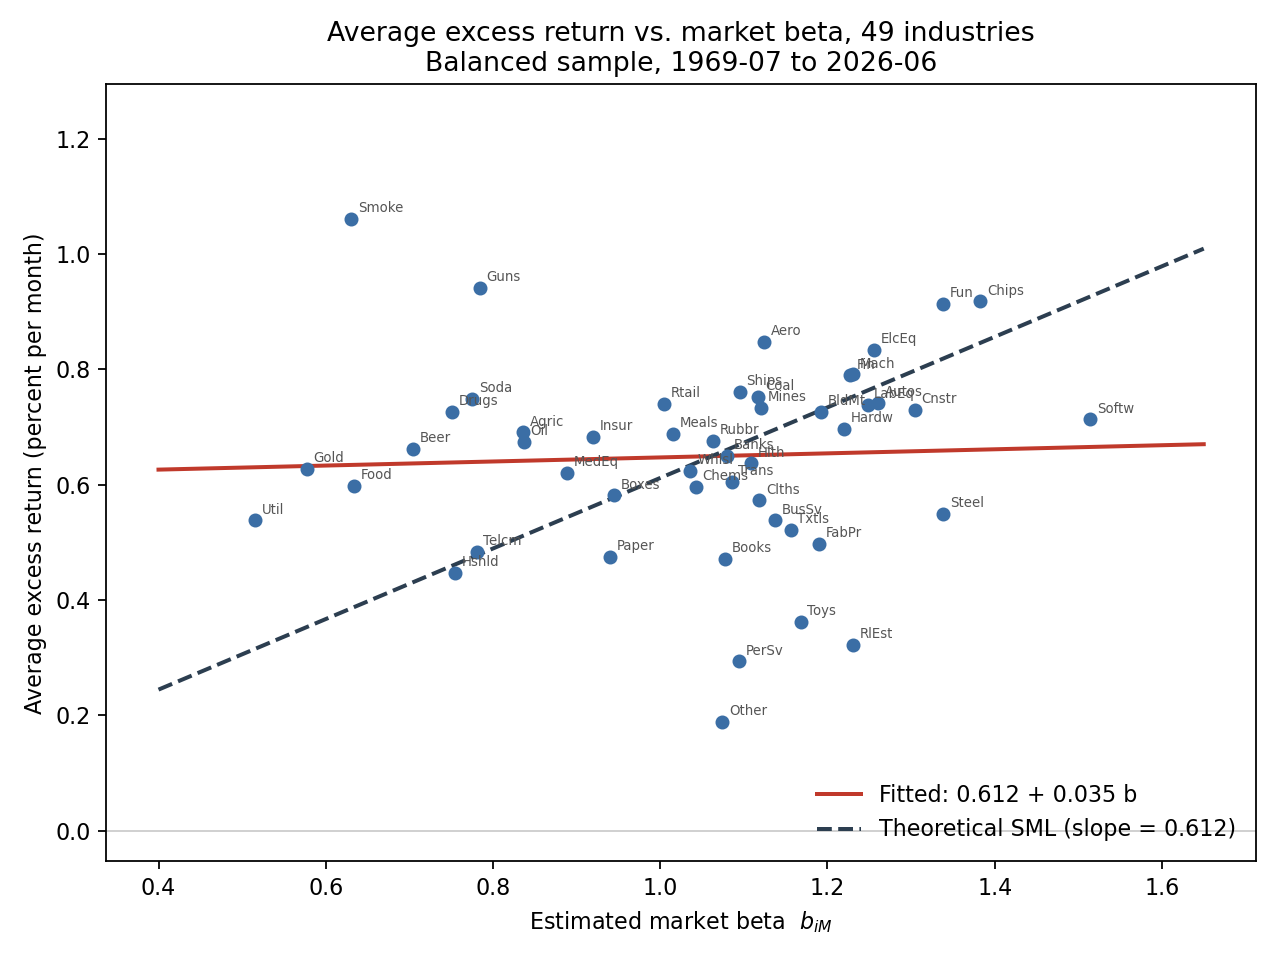
\includegraphics[width=0.72\textwidth]{1d_sml.png}
\caption{Average excess return against estimated beta, 49 industry portfolios,
July 1969 -- June 2026. Solid line: fitted cross-sectional regression,
$\overline{R_i} = 0.612 + 0.035\,b_{iM}$ with $R^2 = 0.002$. Dashed line:
theoretical SML through the origin with slope $0.612$.}
\label{fig:sml}
\end{figure}

\paragraph{Does the plot resemble a positive relationship?} Barely. The fitted
line is almost flat, and beta explains essentially none of the cross-sectional
variation in average returns. Low-beta industries such as Utilities, Gold and
Food earn about as much as high-beta industries such as Software, Chips and
Steel. The vertical scatter at any given beta is much wider than the variation
explained by beta itself, which is visible around $b_{iM} \approx 1.1$, where
average returns range from Other near the bottom of the chart to Ships and Coal
near the top.

\paragraph{What should the plot look like?} Under the CAPM the points should
lie along an upward-sloping straight line. In excess-return space that line
passes through the origin, because a zero-beta portfolio should earn no
premium, and its slope should equal the average market excess return.
Deviations should be small and unsystematic, because beta is supposed to be the
only characteristic that is priced. Instead the fitted line is far too high at
$\beta = 0$ and far too shallow, so it crosses the theoretical line near
$\beta = 1$ and diverges from it in both directions. This is the flat security
market line of part (b) shown graphically.

\paragraph{AI integration: SML prediction.} Asked what the scatter should look
like and what the most common deviation is, the LLM answered that the points
should lie on a line through the origin with slope equal to the market premium,
that the estimated line is typically too flat with a positive intercept, and
that this reflects leverage constraints under Black's zero-beta CAPM, citing
the Frazzini-Pedersen ``betting against beta'' result, and omitted risk factors
such as size and value.

\begin{tight}
\item[(i)] The empirical SML is much flatter than the theoretical one. The
model predicted the direction correctly but understated the degree, describing
a line that still slopes upward, whereas our slope is statistically
indistinguishable from zero.
\item[(ii)] It mentions all three, and its account of the leverage mechanism
is correct. It does not mention errors-in-variables in the estimated betas,
which produces the same flattening for purely statistical reasons, or Roll's
critique, under which a flat line may indicate a poor market proxy rather than
a failed model. The response also referred to our results, so it was not
predicting blind.
\item[(iii)] No. Beta explains almost none of the cross-sectional variation,
and industries with very different betas earn similar average returns.
Utilities and Software have the lowest and highest betas in the sample, yet
their average returns differ by little.
\end{tight}

\subsection{Question (e)}

In the extended regression
\[
R_i = \gamma_0 + \gamma_M \beta_{iM} + \gamma_{size}\ln(\text{size})
+ \gamma_{B/M}\ln(\text{BE/ME}) + \eta_i ,
\]
the CAPM predicts $\gamma_{size} = \gamma_{B/M} = 0$. Expected return depends
only on covariance with the market, so beta is a sufficient statistic and no
other characteristic should have explanatory power once beta is included. Size
and book-to-market are firm characteristics rather than measures of systematic
risk, so they should be priced only if they proxy for beta, and beta is already
controlled for. The predictions for $\gamma_0$ and $\gamma_M$ are unchanged
from part (a).

This regression tests the Fama-French (1992) critique. A significantly negative
$\gamma_{size}$ would indicate a size premium and a significantly positive
$\gamma_{B/M}$ a value premium. Either result rejects the CAPM, regardless of
the estimate of $\gamma_M$.

\subsection{Question (f)}

Using the same fixed betas, we estimate each month
\[
R_{it} = \gamma_{0t} + \gamma_{Mt} b_{iM}
+ \gamma_{size,t}\ln(\text{size}_{t-1})
+ \gamma_{B/M,t}\ln(\text{BE/ME}_{t-1}) + \eta_{it},
\]
with size lagged one month and book-to-market taken from the previous year and
held constant within the year. Eleven negative book-equity observations are
masked, since the logarithm is undefined for them.

\paragraph{Why must the characteristics be lagged?} They must be known to
investors before the return is realized. Size is measured by market
capitalization, which moves with the return itself, so contemporaneous size
would place part of the month's return on both sides of the regression and
create a spurious relationship. Book-to-market has the same problem through its
market value denominator, and annual accounting data is not public until
several months after the fiscal year ends. Lagging makes the regression a test
of whether information available at the start of the month predicts the return
earned over it.

\begin{table}[H]
\centering
\caption{Extended Fama-MacBeth estimates, balanced sample, July 1969 -- June
2026 ($T = 684$), percent per month. The average cross-sectional $R^2$ rises
from $0.09$ in part (b) to $0.18$.}
\small
\begin{tabular}{lrrrl}
\toprule
& Estimate & Std.\ Error & $t$ & CAPM \\
\midrule
$\gamma_0$        & 0.4045 & 0.4988 & 0.81 & 0 \\
$\gamma_M$        & 0.0328 & 0.2595 & 0.13 & 0.6116 \\
$\gamma_{size}$   & 0.0428 & 0.0497 & 0.86 & 0 \\
$\gamma_{B/M}$    & 0.1568 & 0.0805 & 1.95 & 0 \\
\bottomrule
\end{tabular}
\label{tab:fmbext}
\end{table}

\paragraph{Can we reject mean-variance efficiency?} Yes, for the same reason as
in part (b): the slope on beta is still indistinguishable from zero and
significantly below the average market excess return ($t = -2.23$). Adding the
characteristics does not restore a risk-return relationship.

The characteristics themselves give only weak evidence against the CAPM. The
coefficient on book-to-market is positive and marginally significant, which is
consistent with a value premium, while the coefficient on size is small and
insignificant. This is not surprising for industry portfolios, which are not
sorted on these characteristics and therefore show limited cross-sectional
variation in them; the 25 portfolios in Part II provide a sharper test. The
intercept is no longer significant once the characteristics are included, which
suggests the zero-beta return found in part (b) is partly absorbed by
book-to-market rather than being a separate effect. Over the full sample both
characteristics are insignificant and the intercept is significantly positive,
with the rejection again coming from the slope on beta ($t = -2.83$).

\paragraph{AI integration: interpreting size and B/M premia.} The prompt
specified in the assignment asserts significant premia on both characteristics,
which our results do not show, so we ran it as written and then supplied our
actual table, to test whether the model would confirm the premise it was given.
Asked the specified question it identified the rejection at once, noting that
``formally, you're rejecting the joint restriction
$\gamma_{size} = \gamma_{B/M} = 0$, which the CAPM requires,'' and offered
three interpretations: that the characteristics proxy for priced risks a single
market index does not capture, following Fama and French; that ``it's the
characteristics themselves, not the covariance structure, that predict
returns,'' following Daniel and Titman, which points to mispricing; and that a
significant loading is ``also consistent with the market proxy simply being
wrong,'' following Roll.

\begin{tight}
\item[(i)] Yes. It identified the rejection immediately and stated the
restriction the CAPM imposes.
\item[(ii)] Yes, and more fully than required, contrasting the risk-based
reading with the mispricing and invalid-proxy alternatives.
\item[(iii)] Only partly. It noted that the characteristics are known before
the return is earned, but did not make the point that lagging solves the
econometric problem without settling whether the characteristics represent
genuine risk factors.
\end{tight}

Given our actual table it declined to claim a size effect and identified the
beta slope as the main source of rejection, though it misstated $t = 1.95$ as
roughly $5\%$ one-sided and $10\%$ two-sided when the correct values are
$2.6\%$ and $5.2\%$. Asking the model to interpret real output proved a better
test than asking it to explain a result stated in the prompt.


% =====================================================================
\section{Part II: 25 Size and BE/ME Portfolios}
% =====================================================================

\paragraph{Sample.} 1969-07 to 2026-06, $T = 684$, $N = 25$. Estimates and
standard errors: percentage points per month. Mean market excess return:
$0.6116$.

\subsection{Question (1), repeating Part I(b)}

\begin{table}[H]
\centering
\caption{Extended Fama--MacBeth estimates, 25 size and BE/ME portfolios.}
\small
\begin{tabular}{lrrrr}
\toprule
& Estimate & FMB SE & $t$-stat & $p$-value \\
\midrule
\texttt{gamma\_0} & 1.3554 & 0.3998 & 3.390 & 0.0007 \\
\texttt{gamma\_M} & $-0.5758$ & 0.4290 & $-1.342$ & 0.1800 \\
\bottomrule
\end{tabular}
\label{tab:p2b}
\vspace{2pt}\begin{minipage}{0.93\textwidth}\footnotesize
The $t$-statistics test against zero. Average monthly R-squared is $0.2425$ with beta
alone and $0.5288$ for the extended model. For the slope restriction
$E(\gamma_{M,t} - \mathrm{MktRF}_t) = 0$ the mean difference is $-0.8761$ with SE
$0.2629$, giving $t = -3.3320$ and $p = 0.0009$.
\end{minipage}
\end{table}

Using fixed full-period betas and 684 monthly cross-sectional regressions, we
obtain $\bar\gamma_0 = 1.3554$ (FMB SE $= 0.3998$, $t = 3.390$) and
$\bar\gamma_M = -0.5758$ (FMB SE $= 0.4290$, $t = -1.342$), in percent per
month. Standard errors use $\mathrm{sd}(\hat\gamma_{j,t})/\sqrt{T}$.

The significantly positive intercept rejects the zero-intercept restriction.
The slope also falls below the average market excess return of $0.6116\%$; the
difference has $t = -3.0316$ and $p = 0.0025$. These results reject the
Sharpe--Lintner CAPM restrictions and provide evidence against the proxy being
the tangency portfolio for these assets. The insignificant slope relative to
zero is not, by itself, grounds for rejection.

\subsection{Question (1), repeating Part I(c)}

\begin{table}[H]
\centering
\caption{Fama--MacBeth and single cross-sectional regression estimates
compared. Cross-sectional R-squared: $0.1987$. $N = 25$.}
\small
\begin{tabular}{lrrrrrr}
\toprule
& FMB est. & FMB SE & FMB $t$-stat & OLS est. & OLS SE & OLS $t$-stat \\
\midrule
\texttt{gamma\_0} & 1.3554 & 0.3998 & 3.390 & 1.3554 & 0.2619 & 5.1759 \\
\texttt{gamma\_M} & $-0.5758$ & 0.4290 & $-1.342$ & $-0.5758$ & 0.2411 & $-2.3884$ \\
\bottomrule
\end{tabular}
\label{tab:p2c}
\end{table}

The single cross-sectional regression gives the same coefficients as
Fama--MacBeth: $\gamma_0 = 1.3554$ and $\gamma_M = -0.5758$, with
$R^2 = 0.1987$ and $N = 25$. Equality follows because the panel is balanced and
the regressors are fixed: averaging monthly OLS coefficients is equivalent to
regressing average returns on the same betas.

The OLS standard errors, $0.2619$ and $0.2411$, are smaller than the FMB
standard errors, $0.3998$ and $0.4290$. OLS measures dispersion around the
average-return regression, whereas FMB measures variation in monthly
coefficient estimates. FMB is preferable for inference on average premia here
because it incorporates that time-series variation and accommodates
contemporaneous correlation across portfolio returns. It does not eliminate
error from estimated betas.

\subsection{Question (1), repeating Part I(d)}

\begin{figure}[H]
\centering
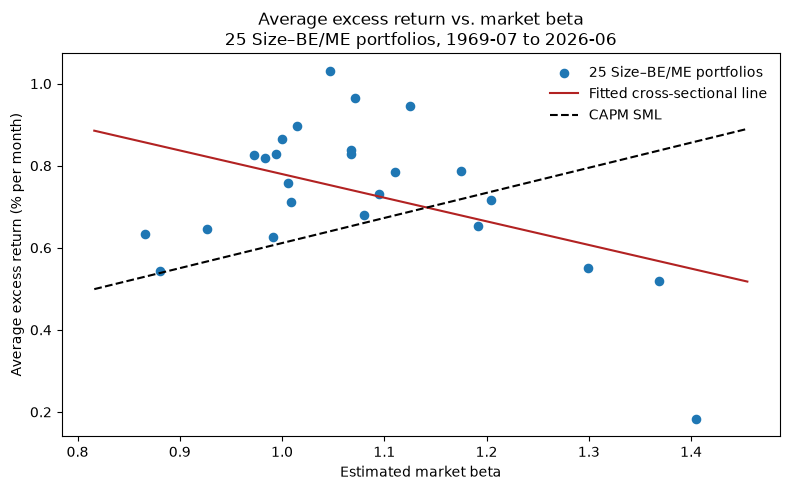
\includegraphics[width=0.78\textwidth]{Part2/figs/p2_1d_sml.png}
\caption{Average excess return against estimated market beta, 25
size--BE/ME portfolios. Fitted line: $1.3554 + (-0.5758) \times$ beta.
CAPM SML: $0.6116 \times$ beta. Cross-sectional R-squared: $0.1987$.}
\label{fig:p2d}
\end{figure}

The plot shows a negative fitted relationship:
\[
R^e_i = 1.3554 - 0.5758\,\hat\beta_{iM}.
\]
The CAPM instead predicts a line through the origin with positive slope
$0.6116$. The portfolios are widely scattered around the fitted line, with
$R^2 = 0.1987$, so market beta explains little of their average-return
variation. The plot is inconsistent with the predicted SML, although visual
evidence alone is not a formal statistical test.

\subsection{Question (1), repeating Part I(f)}

\begin{table}[H]
\centering
\caption{Extended Fama--MacBeth estimates ($t$-statistics test zero). Average
monthly R-squared, beta only: $0.2425$; extended: $0.5288$. Slope restriction
$E(\gamma_{M,t} - \mathrm{MktRF}_t) = 0$: mean difference $= -0.8761$,
SE $= 0.2629$, $t = -3.3320$, $p = 0.0009$.}
\small
\begin{tabular}{lrrrr}
\toprule
& Estimate & FMB SE & $t$-stat & $p$-value \\
\midrule
\texttt{gamma\_0}    & 1.1539 & 0.3392 & 3.4017 & 0.0007 \\
\texttt{gamma\_M}    & $-0.2646$ & 0.3134 & $-0.8442$ & 0.3989 \\
\texttt{gamma\_size} & $-0.0194$ & 0.0302 & $-0.6428$ & 0.5206 \\
\texttt{gamma\_BM}   & 0.1573 & 0.0747 & 2.1055 & 0.0356 \\
\bottomrule
\end{tabular}
\label{tab:p2f}
\end{table}

With lagged characteristics included, the estimates are $\gamma_0 = 1.1539$
($t = 3.4017$), $\gamma_M = -0.2646$ ($t = -0.8442$),
$\gamma_{size} = -0.0194$ ($t = -0.6428$), and $\gamma_{B/M} = 0.1573$
($t = 2.1055$). Book-to-market has a positive premium significant at $5\%$,
while size is insignificant. Average monthly cross-sectional $R^2$ rises from
$0.2425$ to $0.5288$.

The positive book-to-market premium contradicts the CAPM prediction that
characteristics have no additional explanatory power after controlling for
beta. The intercept remains significantly positive, and the beta premium
remains below the market premium ($t = -3.3320$, $p = 0.0009$). Thus, adding
characteristics does not restore the Sharpe--Lintner CAPM restrictions.

Size is lagged one month and BE/ME uses the previous year's value, held
constant within each year. This follows the assignment's information-timing
convention and avoids using contemporaneous characteristics, though actual
accounting-data availability would require publication dates.

\subsection{Question (2)}

\paragraph{2(a).} Using the 684 monthly observations from July 1969 to June
2026, we calculate the sample mean vector $\hat\mu$ and covariance matrix
$\hat\Sigma$ of the 25 portfolios' excess returns. The tangency weights are
\[
w_T = \frac{\hat\Sigma^{-1}\hat\mu}{\mathbf{1}'\hat\Sigma^{-1}\hat\mu}.
\]
The weights sum to one, with short selling allowed.

\begin{table}[H]
\centering
\caption{In-sample tangency weights and tangency betas.}
\small
\begin{tabular}{lrrlrr}
\toprule
Portfolio & Weight & Tang.\ beta & Portfolio & Weight & Tang.\ beta \\
\midrule
Size1\_BM1 & $-1.9858$ & 0.0725 & Size3\_BM4 & $-0.2411$ & 0.3253 \\
Size1\_BM2 & 0.6508 & 0.2841 & Size3\_BM5 & 0.2578 & 0.3834 \\
Size1\_BM3 & $-0.0034$ & 0.2903 & Size4\_BM1 & 1.1460 & 0.2595 \\
Size1\_BM4 & 0.9189 & 0.3563 & Size4\_BM2 & $-0.6837$ & 0.2694 \\
Size1\_BM5 & 0.9936 & 0.4092 & Size4\_BM3 & $-0.0040$ & 0.3006 \\
Size2\_BM1 & $-0.2076$ & 0.2061 & Size4\_BM4 & 0.4626 & 0.3274 \\
Size2\_BM2 & 0.8054 & 0.3119 & Size4\_BM5 & $-0.1819$ & 0.3330 \\
Size2\_BM3 & 0.2286 & 0.3289 & Size5\_BM1 & 0.7176 & 0.2484 \\
Size2\_BM4 & $-0.0409$ & 0.3435 & Size5\_BM2 & 0.0421 & 0.2559 \\
Size2\_BM5 & $-0.4743$ & 0.3749 & Size5\_BM3 & 0.5150 & 0.2519 \\
Size3\_BM1 & $-0.6186$ & 0.2183 & Size5\_BM4 & $-1.0900$ & 0.2154 \\
Size3\_BM2 & 0.0531 & 0.3109 & Size5\_BM5 & 0.4014 & 0.3288 \\
Size3\_BM3 & $-0.6615$ & 0.2819 &            &         &        \\
\bottomrule
\end{tabular}
\label{tab:p2w}
\vspace{2pt}\begin{minipage}{0.93\textwidth}\footnotesize
Weights are fractions of portfolio value and size and BE/ME groups increase from 1 to 5.
Sum of weights $1.000000$; gross exposure $13.3859$; mean excess return $2.5204\%$ per
month; monthly volatility $6.0461\%$; monthly Sharpe ratio $0.4169$; weighted average
beta $1.000000$.
\end{minipage}
\end{table}

Gross exposure,
\[
\sum_i |w_i|,
\]
is $13.3859$, indicating substantial offsetting long and short positions.

\paragraph{2(b) Returns, betas, and cross-sectional results.} We construct the
tangency portfolio's monthly excess return using the same fixed weights
throughout:
\[
R^e_{T,t} = \sum_{i=1}^{25} w_{T,i} R^e_{i,t}.
\]
Its average excess return is $2.5204\%$ per month, monthly volatility is
$6.0461\%$, and the monthly Sharpe ratio is $0.4169$.

We estimate each portfolio's beta by regressing its excess returns on
$R^e_{T,t}$, including an intercept. Regressing average excess returns on these
new betas gives
\[
R^e_i \approx 0 + 2.5204\,\hat\beta_{i,T}, \qquad R^2 = 1, \qquad N = 25.
\]
The estimated intercept is effectively zero, while the slope equals the
tangency portfolio's average excess return. All 25 portfolios lie essentially
on the theoretical SML, so the fitted and theoretical lines overlap. The OLS
standard errors are effectively zero; the resulting $t$-statistics are not
economically meaningful because the fit is mechanically exact.

\begin{table}[H]
\centering
\caption{Cross-sectional regression using the in-sample tangency portfolio as the market proxy.}
\small
\begin{tabular}{lrrr}
\toprule
& Estimate & OLS SE & $t$-stat \\
\midrule
\texttt{gamma\_0} & $4.83988\times10^{-15}$ & $4.34718\times10^{-15}$ & 1.11334 \\
\texttt{gamma\_M} & 2.52036 & $1.45191\times10^{-14}$ & $1.7359\times10^{14}$ \\
\bottomrule
\end{tabular}
\label{tab:p2q2}
\vspace{2pt}\begin{minipage}{0.93\textwidth}\footnotesize
Cross-sectional R-squared $1.000000$, $N = 25$. Mean tangency excess return $2.5204\%$ per
month and maximum absolute residual $9.659\times10^{-15}$. Fitted line
$0.0000 + (2.5204)\times$ beta; CAPM SML $2.5204\times$ beta.
\end{minipage}
\end{table}

\begin{figure}[H]
\centering
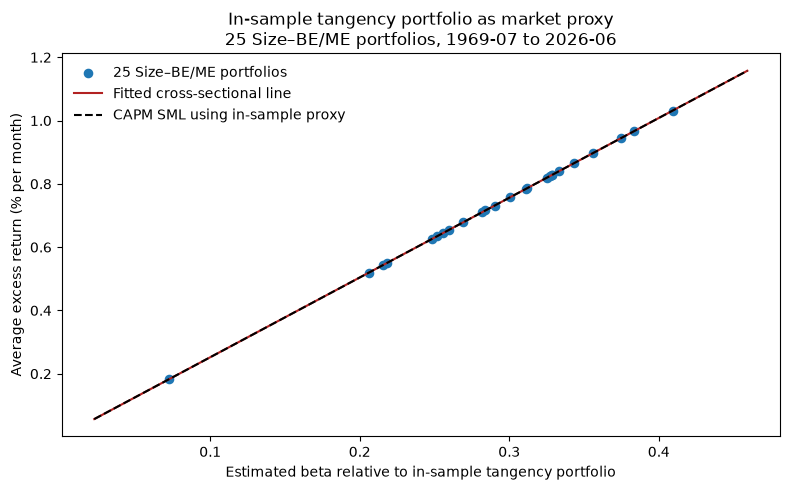
\includegraphics[width=0.78\textwidth]{Part2/figs/p2_q2_insample.png}
\caption{Average excess return against beta estimated against the in-sample
tangency portfolio. Fitted line: $0.0000 + (2.5204)\times$ beta. CAPM SML:
$2.5204\times$ beta.}
\label{fig:p2q2}
\end{figure}

\paragraph{2(c).} This perfect fit does not independently support the CAPM. The
tangency portfolio is constructed to be mean--variance efficient using the same
assets and observations used in the regression. Its weights satisfy
\[
w_T \propto \hat\Sigma^{-1}\hat\mu,
\]
which implies
\[
\hat\mu_i = \hat\beta_{i,T}\,\hat\mu_T .
\]
Thus, the zero intercept, matching slope, and perfect fit follow from portfolio
mathematics.

This illustrates Roll's critique: CAPM tests depend on whether the chosen
market proxy is mean--variance efficient. The true market portfolio includes
all wealth and is not directly observable. Rejecting the CAPM with a particular
proxy could therefore reflect a poor proxy, while obtaining a perfect fit with
a deliberately constructed tangency portfolio does not establish that the true
market portfolio is efficient.

\subsection{Question (3)}

\paragraph{3(a).} Sample 1 contains odd-numbered months in even years and
even-numbered months in odd years, giving 342 observations. Using only these
observations, we estimate the mean vector and covariance matrix of excess
returns and calculate
\[
w_1 = \frac{\hat\Sigma_1^{-1}\hat\mu_1}{\mathbf{1}'\hat\Sigma_1^{-1}\hat\mu_1}.
\]
The weights sum to 1, with gross exposure $\sum_i |w_{1,i}| = 15.4800$ and
individual weights ranging from $-1.6671$ to $1.4736$. We hold these weights
fixed and apply them to the 342 months in Sample 2. These returns are out of
sample because none of the evaluation observations were used to estimate the
weights.

\paragraph{3(b).} Sample 2 contains even-numbered months in even years and
odd-numbered months in odd years, also giving 342 observations. We estimate a
separate tangency portfolio using only Sample 2's mean vector and covariance
matrix, with the same normalization.

These weights sum to 1, have gross exposure of $17.2082$, and range from
$-2.4853$ to $1.3680$. We then apply them, unchanged, to Sample 1 returns. This
reverses the estimation and evaluation samples, ensuring that neither half is
evaluated using weights estimated from itself. The checks confirm that the
samples do not overlap and together cover all 684 months.

\begin{table}[H]
\centering
\caption{Out-of-sample tangency weights. Sample 1: 342 months; Sample 2: 342
months; total 684 months, no overlap and complete coverage.}
\small
\begin{tabular}{llrrrr}
\toprule
Estimated from & Applied to & Weight sum & Gross exposure & Min weight & Max weight \\
\midrule
Sample 1 & Sample 2 & 1.0 & 15.4800 & $-1.6671$ & 1.4736 \\
Sample 2 & Sample 1 & 1.0 & 17.2082 & $-2.4853$ & 1.3680 \\
\bottomrule
\end{tabular}
\label{tab:p2oosw}
\end{table}

\paragraph{3(c).} We combine Sample 1 returns generated with $w_2$ and Sample 2
returns generated with $w_1$, then sort them chronologically. The resulting OOS
tangency series covers July 1969--June 2026 and has a mean excess return of
$1.9754\%$ per month, monthly volatility of $7.0300\%$, and monthly Sharpe
ratio of $0.2810$.

We use this combined excess-return series as the market proxy and estimate each
portfolio's beta through a full-period time-series regression with an
intercept. The cross-sectional regression of average excess returns on these
betas is
\[
R^e_i = 0.0684 + 3.2851\,\hat\beta_{i,\mathrm{OOS}} + \hat\eta_i .
\]

\begin{table}[H]
\centering
\caption{Cross-sectional regression using the out-of-sample tangency portfolio as the market proxy.}
\small
\begin{tabular}{lrrr}
\toprule
Coefficient & Estimate & OLS standard error & $t$-statistic \\
\midrule
$\gamma_0$ & 0.0684 & 0.0228 & 2.9930 \\
$\gamma_M$ & 3.2851 & 0.1091 & 30.1058 \\
\bottomrule
\end{tabular}
\label{tab:p2q3}
\vspace{2pt}\begin{minipage}{0.93\textwidth}\footnotesize
Returns are in percent per month. The regression has $R^2 = 0.9753$ and $N = 25$, and the
mean out-of-sample market excess return is $1.9754\%$ per month.
\end{minipage}
\end{table}

\begin{figure}[H]
\centering
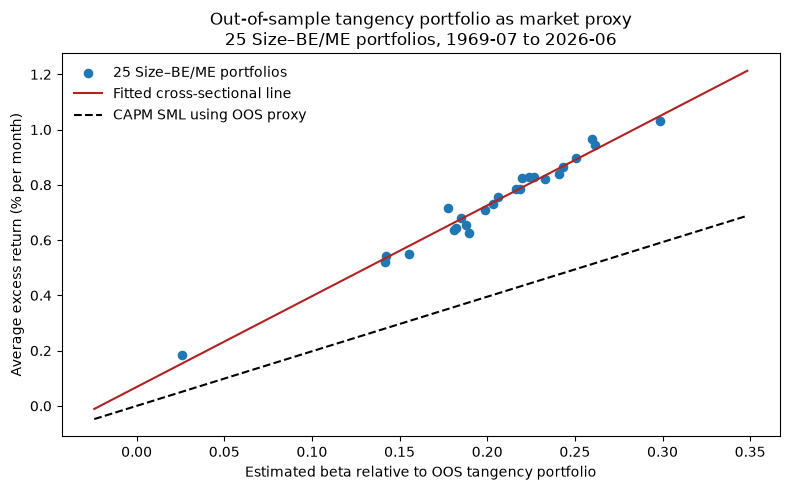
\includegraphics[width=0.78\textwidth]{Part2/figs/p2_q3_oos.png}
\caption{Average excess return against beta estimated against the
out-of-sample tangency portfolio. Fitted line: $0.0684 + (3.2851)\times$ beta.
CAPM SML: $1.9754\times$ beta.}
\label{fig:p2q3}
\end{figure}

The plot shows a strong positive relationship: the portfolios cluster closely
around the fitted line, which explains $97.53\%$ of the cross-sectional
variation in average excess returns. However, the fitted line lies above the
theoretical SML, whose intercept is zero and slope is $1.9754$. Thus, a close
fit to the estimated line does not establish that the CAPM restrictions hold.
The reported slope $t$-statistic tests equality to zero, not equality to
$1.9754$.

Each month's return is excluded from the sample used to estimate its portfolio
weights. Because the two samples are interleaved in time, this is a
held-out-sample exercise rather than a strictly forward-looking trading
backtest.

\subsection{Question (4)}

\paragraph{1. Comparing the results.}

\begin{table}[H]
\centering
\caption{In-sample and out-of-sample tangency proxies compared.}
\small
\begin{tabular}{lrr}
\toprule
Statistic & Q2: In-sample & Q3: Out-of-sample \\
\midrule
$\gamma_0$ (SE, $t$) & $4.84\times10^{-15}$ & 0.0684 \\
 & ($4.35\times10^{-15}$, $t = 1.11$) & (0.0228, $t = 2.99$) \\
$\gamma_M$ (SE, $t$) & 2.5204 & 3.2851 \\
 & ($1.45\times10^{-14}$, $t = 1.74\times10^{14}$) & (0.1091, $t = 30.11$) \\
Proxy mean excess return (CAPM slope) & 2.5204 & 1.9754 \\
$\gamma_M \div$ proxy premium & 1.00 & 1.66 \\
Cross-sectional $R^2$ & 1.000000 & 0.9753 \\
Max absolute residual & $9.66\times10^{-15}$ & not reported \\
Proxy Sharpe ratio (monthly) & 0.4169 & 0.2810 \\
\bottomrule
\end{tabular}
\label{tab:p2q4}
\end{table}

\begin{tight}
\item $\gamma_0$: In Q2 the intercept is zero to machine precision. The
$t = 1.11$ is rounding noise, not a meaningful test. In Q3 the intercept is
$0.0684\%$ per month, about $0.82\%$ per year, with $t = 2.99$, indicating a
statistically significant common pricing error across the 25 portfolios.

\item $\gamma_M$: In Q2 the slope equals the proxy's premium exactly,
$2.5204$. In Q3 the slope is $3.2851$, about $1.66$ times the proxy premium of
$1.9754$. The raw slopes should not be compared directly across Q2 and Q3
because each set of betas is measured against a different proxy. What matters
for the CAPM is whether the slope equals that proxy's own premium. It does in
Q2 but not in Q3.

\item Standard errors: Q2's standard errors are essentially zero because the
regression residuals are essentially zero, so the enormous slope $t$-statistic
is not economically informative. Q3's $t$-statistics use ordinary
cross-sectional OLS standard errors, which do not account for beta-estimation
error or cross-portfolio dependence. Also, $t = 30.11$ tests $\gamma_M = 0$,
not the CAPM restriction $\gamma_M = 1.9754$.

\item SML shape: In Q2 the fitted line,
$R^e_i = 0.0000 + 2.5204\beta_i$,
and the theoretical SML are the same line. In Q3 the fitted line,
$R^e_i = 0.0684 + 3.2851\beta_i$,
has both a higher intercept and a steeper slope than the theoretical SML,
$R^e_i = 1.9754\beta_i$. Thus, for positive betas, the fitted Q3 line lies
above the theoretical SML.

\item Which is cleaner? Q2 fits the CAPM restrictions mechanically: the
intercept is zero, the slope equals the proxy premium, and $R^2 = 1$. Both Q2
and Q3 fit much better than the value-weighted market proxy in Part I, where
$\gamma_0 = 1.3554$, $\gamma_M = -0.5758$, and $R^2 = 0.1987$.
\end{tight}

\paragraph{2. Why Q2 and Q3 differ, and the link to Roll (1977).}

\textbf{The in-sample proxy is efficient by construction.} Using excess
returns, the tangency weights are
\[
w_T = \frac{\hat\Sigma^{-1}\hat\mu}{\mathbf{1}'\hat\Sigma^{-1}\hat\mu}.
\]
Let
\[
c = \mathbf{1}'\hat\Sigma^{-1}\hat\mu.
\]
Then the result follows in four steps:
\begin{enumerate}\setlength{\itemsep}{2pt}\setlength{\topsep}{3pt}
\item Rearranging the tangency-weight formula gives
$\hat\Sigma w_T = \hat\mu / c$.
\item $\hat\Sigma w_T$ is the vector of sample covariances between each
portfolio and the tangency portfolio:
$\widehat{\mathrm{Cov}}(R_i, R_T)$.
\item The tangency portfolio's variance is
$w_T'\hat\Sigma w_T = \hat\mu_T / c$.
\item Therefore,
\[
\hat\beta_i = \frac{\widehat{\mathrm{Cov}}(R_i, R_T)}
{\widehat{\mathrm{Var}}(R_T)} = \frac{\hat\mu_i}{\hat\mu_T},
\qquad\text{which implies}\qquad
\hat\mu_i = \hat\beta_i \hat\mu_T .
\]
\end{enumerate}
This identity holds for every portfolio.

Q2 estimates the weights using the same 684 months and the same 25 portfolios
that are subsequently used in the CAPM test. Because the OLS betas are also
based on the same sample covariances and variances, the beta-pricing identity
must hold essentially exactly. The maximum residual of $9.66\times10^{-15}$
confirms this.

\textbf{Why the CAPM can look successful even when the market is mismeasured.}
Roll's critique is that an empirical CAPM test is fundamentally a test of
whether the chosen market proxy is mean-variance efficient. The true CAPM
market portfolio contains all relevant wealth and cannot be directly observed.

The results illustrate the problem. With the observable value-weighted market
proxy in Part I, the CAPM performs poorly. With a proxy constructed directly
from the test assets in Q2, the fit becomes perfect. Nothing about the true
market changed; only the proxy changed.

Therefore, Q2's apparent success mainly shows that the proxy was constructed to
be mean-variance efficient relative to these 25 portfolios in this sample. A
perfect fit does not independently establish that the true market portfolio is
efficient, while rejection using another proxy could reflect proxy error rather
than failure of the CAPM itself.

\textbf{Why the out-of-sample version is more informative.} In Q3, each month's
proxy return uses tangency weights estimated from the opposite half of the
data. Therefore, the means and covariances used to construct the proxy are no
longer the same moments used to evaluate it. The exact in-sample identity above
no longer has to hold.

Estimation error therefore becomes important:
\begin{tight}
\item Inverting the $25\times25$ covariance matrix in
$\hat\Sigma^{-1}\hat\mu$
can magnify estimation noise.
\item This produces large long and short positions. Gross exposure is $15.48$
and $17.21$ in the two estimation samples, with individual weights ranging
roughly from $-2.4853$ to $1.4736$.
\item Weights optimized using one half of the data may partly fit noise
specific to that half. When applied to the other half, performance
deteriorates. The proxy mean falls from $2.5204\%$ to $1.9754\%$ per month,
volatility rises from $6.0461\%$ to $7.0300\%$, and the monthly Sharpe ratio
falls from $0.4169$ to $0.2810$.
\item Because the OOS proxy is no longer guaranteed to lie on the
evaluation-sample mean-variance frontier, pricing errors appear:
$\gamma_0 > 0$, the fitted slope differs from the proxy premium, and
$R^2 < 1$.
\end{tight}

The remaining high $R^2$ of $0.9753$ indicates that the beta-return relation
remains strong out of sample, even though the exact in-sample CAPM identity
disappears.

Limits of the Q3 test:
\begin{tight}
\item The two samples alternate months and therefore span the same broad
economic periods, so this is a relatively mild out-of-sample test.
\item The second-pass average returns and betas are calculated using the
combined sample, so the design is not equivalent to a completely separate
future holdout period.
\item The OOS proxy is still constructed from the same 25 test portfolios
rather than from the true aggregate market portfolio. Therefore, Q3 makes the
test more informative but does not eliminate Roll's critique.
\end{tight}

\paragraph{3. Evaluating the LLM explanation.}

\textbf{1. Did it predict a steeper SML and lower pricing errors?} Partly.

The LLM correctly predicted that an in-sample tangency proxy would generate
small pricing errors and a very strong beta-return relationship. It actually
understated the strength of the result: it called the exercise ``almost
tautological,'' while Q2 produces an essentially exact fit with
$R^2 = 1.000000$.

However, it did not explicitly predict a steeper SML. In fact, ``steeper'' is
not the key criterion. Q3's fitted slope, $3.2851$, is numerically steeper than
Q2's $2.5204$. The important CAPM restriction is instead whether the fitted
slope equals the proxy's own mean excess return. That equality holds exactly in
Q2 but fails in Q3.

\textbf{2. Did it explain why the portfolio is efficient by construction?} Yes.
This is the strongest part of the LLM explanation.

It correctly argues that the tangency first-order condition implies
\[
\mu - r_f\mathbf{1} \propto \Sigma w_T ,
\]
and recognizes that $\Sigma w_T$ is the vector of covariances between each test
asset and the tangency portfolio. This leads directly to beta pricing.

There are two minor precision issues:
\begin{tight}
\item It skips the intermediate step needed to determine the proportionality
constant. Premultiplying by $w_T'$ gives the connection between the constant,
the tangency portfolio premium, and its variance.
\item It writes the result using population expectations such as $E[R_i]$,
whereas the exact identity here is an \emph{in-sample} identity involving
sample moments, such as $\hat\mu_i$. This distinction explains why the Q2 fit
is exact in the observed sample but need not hold out of sample.
\end{tight}

\textbf{3. Did it anticipate why the out-of-sample results could deteriorate?}
In general terms, yes. The LLM correctly explained that moments in the
evaluation sample need not equal the moments used to estimate the weights, so
mean-variance efficiency is no longer guaranteed.

However, its explanation was less complete about the empirical pattern observed
in Q3. It did not emphasize:
\begin{tight}
\item estimation error amplified by $\hat\Sigma^{-1}$;
\item the resulting extreme leveraged weights;
\item the lower out-of-sample Sharpe ratio;
\item the positive intercept and slope exceeding the proxy premium;
\item the fact that $R^2$ nevertheless remains high at $0.9753$;
\item the exact two-way sample-splitting procedure used in Q3;
\item or the fact that the OOS proxy is still not the true market portfolio, so
Roll's critique remains relevant.
\end{tight}

Overall, the LLM's explanation is conceptually correct and explains the exact
in-sample fit in Q2 well. It is less complete in explaining the magnitude and
specific pattern of the deterioration observed in Q3.


% =====================================================================
\section{AI Exercise 1 --- Stress-Testing LLM Knowledge of Fama-MacBeth
Econometrics}
% =====================================================================

LLM used: ChatGPT. The three questions were asked one at a time in a single
conversation. Full responses:
\href{https://chatgpt.com/share/6ab8a8ae-5c10-83ea-a8ee-345b18c411cf}{shared transcript}.

\subsection{Question 1: Shanken (1992) Correction}

\paragraph{Prompt.} What is the Shanken (1992) correction and when should it be
applied to Fama-MacBeth standard errors?

\paragraph{Summary of the LLM's Answer.} The LLM explained that the second-pass
Fama-MacBeth regression uses estimated betas, but conventional Fama-MacBeth
standard errors treat them as known, so they overstate the precision of the
estimated risk premia. It gave Shanken's adjusted covariance matrix,
$V_{Shanken} = (1+c)\Omega + \Sigma_f^*$ with $c = \lambda'\Sigma_f^{-1}\lambda$,
compared with the conventional $V_{FM} = \Omega + \Sigma_f^*$, so corrected
standard errors are larger and $t$-statistics smaller. It said the correction
should be applied when the second-pass regressors are estimated betas, but
generally not when they are observed characteristics such as size or
book-to-market, and that it matters more when betas are noisy or the time series
used to estimate them is short. It also noted that Shanken's result assumes
conditional homoskedasticity and that the correction is different from
Newey-West, which addresses serial correlation and heteroskedasticity.

\paragraph{Evaluation.} The answer is mostly correct. The LLM correctly
identifies the source of the problem (estimated betas treated as known), the
direction of the error in conventional standard errors (too small), when the
correction applies and when it does not, and the difference from Newey-West.
Its general formula is consistent with the assignment's answer: with a single
market factor, $c = \lambda^2/\sigma_M^2$, so the correction inflates the
conventional variance by $(1 + \lambda^2/\sigma_M^2)$. However, it never
reduces the formula to this one-factor case, so the key result is left
implicit. Its statement that the correction matters more when the
beta-estimation sample is short is imprecise: the size of the correction
relative to the conventional standard error depends on $c$, the squared Sharpe
ratio of the factor, not on the sample length. It also does not mention that
$c$ is small for a monthly market factor, so the correction is usually modest
in practice.

\paragraph{My Correction.} In the one-factor case, $c = \lambda^2/\sigma_M^2$,
so the Shanken correction inflates the conventional Fama-MacBeth variance
(apart from the factor-variance term) by $1 + \lambda^2/\sigma_M^2$, and
because this term is the squared Sharpe ratio of the market rather than a
function of sample length, it is usually small for monthly market data.

\subsection{Question 2: Errors-in-Variables}

\paragraph{Prompt.} Does the Fama-MacBeth procedure fully solve the
errors-in-variables problem caused by using estimated betas as regressors? If
not, what bias remains?

\paragraph{Summary of the LLM's Answer.} The LLM said Fama-MacBeth does not
fully solve the errors-in-variables problem: the same noisy estimated betas are
the regressors in every monthly cross-sectional regression, so averaging the
monthly risk-premium estimates does not remove the measurement error. With one
factor and classical measurement error, the estimated premium is attenuated
toward zero by the factor
$\text{Var}(\beta)/[\text{Var}(\beta)+\text{Var}(e)]$; with several factors,
the estimates are jointly distorted and not every coefficient is necessarily
biased toward zero. It added that the Shanken correction adjusts the standard
errors but does not remove the bias in the coefficients, and that the bias
shrinks as the first-stage beta estimates become more precise.

\paragraph{Evaluation.} The answer is correct but incomplete. The LLM correctly
explains why averaging does not remove the measurement error, identifies
attenuation bias toward zero in the one-factor case, gives the attenuation
factor, notes that the multi-factor case cannot always be signed, and usefully
distinguishes the bias (which Shanken does not fix) from the standard errors
(which it does). However, it does not state that the bias persists even in
large samples, meaning that adding more assets does not reduce it. It also does
not mention that attenuation of the slope biases the intercept upward,
producing a flatter estimated security market line, or that grouping stocks
into portfolios is the standard way to reduce beta measurement error.

\paragraph{My Correction.} Because the same noisy betas enter every monthly
regression, the estimated market premium $\gamma_M$ is attenuated toward zero,
and with a positive premium the intercept is biased upward, even when the
number of assets is large, so the bias can only be reduced by estimating betas
more precisely, for example by using portfolios.

\subsection{Question 3: Serial Correlation in Monthly Gamma Estimates}

\paragraph{Prompt.} In a FMB regression where the same betas are used every
month, are the monthly gamma estimates serially uncorrelated? Does this matter
for the standard error calculation?

\paragraph{Summary of the LLM's Answer.} The LLM said that using the same betas
every month does not by itself make the monthly gamma estimates serially
correlated. Because the betas are fixed, each month's estimate is
$\hat\gamma_t = (\hat B'\hat B)^{-1}\hat B' R_t$, so the gammas are serially
correlated only if returns or regression disturbances are correlated over time,
which can happen in real data. The usual standard error
$s(\hat\gamma_t)/\sqrt{T}$ assumes no serial correlation; if the gammas are
positively autocorrelated, it is usually too small and the $t$-statistics too
large, and Newey-West/HAC standard errors should be used. It again
distinguished Newey-West (serial correlation) from Shanken (estimated betas).

\paragraph{Evaluation.} The answer is mostly correct. It identifies the
mechanism behind the assignment's answer: because the betas are fixed, each
$\hat\gamma_t$ is a fixed linear combination of that month's returns, so the
gammas inherit whatever autocorrelation the returns have. It also correctly
explains why this matters, the direction of the resulting error in the standard
errors, and the Newey-West remedy. Its framing (fixed betas do not by
themselves cause serial correlation) differs in emphasis from the assignment's
(fixed betas are why the gammas inherit return autocorrelation), but the two
are consistent. However, it does not address magnitude: it presents Newey-West
as the remedy without noting that autocorrelation in monthly returns, and
therefore in the gammas, is typically mild.

\paragraph{My Correction.} Because the betas are fixed, each monthly gamma is a
fixed-weight portfolio return, so the gammas are serially correlated only to
the extent that returns are, which is typically mild for monthly data, so the
usual $s(\hat\gamma_t)/\sqrt{T}$ standard error is usually adequate, with
Newey-West as a robustness check.


% =====================================================================
\section{AI Exercise 2 --- Predicting Cross-Sectional Deviations from the SML}
% =====================================================================

We asked an LLM which of the 49 industries it expected to fall above, below and
near the security market line, and recorded its answer before comparing it with
our results from Question (d).

\paragraph{(a) The LLM's predictions.}
\begin{tight}
\item \textit{Above the line:} Tobacco, Utilities, Beer \& Liquor / Food.
\item \textit{Below the line:} Coal / Mining, Computers / Electronic Equipment
/ Semiconductors, Autos / Steel.
\item \textit{Near the line:} Wholesale / Retail, Transportation, Financials /
Business Services.
\end{tight}

Its reasoning was the low-beta anomaly. Defensive industries have low beta but
still earn competitive returns, so they plot above the line, while cyclical
industries have high beta without the returns to match. It added a sin-stock
premium for tobacco and a glamour effect for technology. It stated that these
were predictions from documented patterns, not calculations from the data.

\paragraph{(b) What the plot shows.} Deviations are measured from the
theoretical SML in Figure~\ref{fig:sml}, as
$\overline{R_i} - \bar{R}_M^{e}\,b_{iM}$.

\begin{table}[H]
\centering
\caption{Largest deviations from the theoretical security market line, balanced
sample, percent per month. A positive value means the industry earned more than
its beta implies.}
\small
\begin{tabular}{lrlrlr}
\toprule
\multicolumn{2}{c}{Above} & \multicolumn{2}{c}{Below}
& \multicolumn{2}{c}{Near} \\
\cmidrule(lr){1-2}\cmidrule(lr){3-4}\cmidrule(lr){5-6}
Smoke & $+0.675$ & Other & $-0.468$ & BldMt & $-0.003$ \\
Guns  & $+0.461$ & RlEst & $-0.429$ & Boxes & $+0.004$ \\
Soda  & $+0.274$ & PerSv & $-0.376$ & Telcm & $+0.006$ \\
\bottomrule
\end{tabular}
\label{tab:dev}
\end{table}

\paragraph{(c) How accurate were the predictions?} The above-line predictions
were accurate. All three industries plot above the line, and Tobacco is the
largest positive deviation in the sample. The near-line predictions were also
reasonable: Wholesale, Transportation and Financials all sit close to the line,
though none is among the three closest.

The below-line predictions were mostly wrong. Coal and Mining plot slightly
above the line rather than below it. Of the technology group, only Software is
clearly below, while Chips and Electronic Equipment are above. Only Steel was
placed correctly, and none of the three largest negative deviations was
anticipated.

This asymmetry is explained by how the model reasoned. It used beta alone,
predicting that low-beta industries plot above the line and high-beta
industries plot below. Because the estimated line is so flat, the first half of
this is almost automatic, since nearly any low-beta industry lands above the
theoretical SML. That is why the above-line predictions worked. The below-line
predictions needed more, because high beta is not sufficient: Chips and
Electronic Equipment have high betas but earned enough to stay above the line.
The industries that actually fall furthest below have betas near the sample
average and unusually low returns, which reflects industry-specific weakness
rather than a risk story the model could infer.

Its caveat about technology was partly right. It predicted technology would
fall below the line but noted that recent data might reverse this. The reversal
is what we observe for Chips and Electronic Equipment, though not for Software.


% =====================================================================
\section{AI Exercise 3 --- Literature Synthesis and Historical Context}
% =====================================================================

\subsection{3(a)}

\begin{table}[H]
\centering
\caption{Fama-MacBeth estimates reported in Part I(b).}
\small
\begin{tabular}{llrrrr}
\toprule
Sample & Parameter & Estimate & Standard error & $t$ & $p$ \\
\midrule
July 1969--June 2026 & $\gamma_0$ & 0.6119 & 0.2191 & 2.79 & 0.005 \\
July 1969--June 2026 & $\gamma_M$ & 0.0352 & 0.2725 & 0.13 & 0.897 \\
July 1926--June 2026 & $\gamma_0$ & 0.5160 & 0.1714 & 3.01 & 0.003 \\
July 1926--June 2026 & $\gamma_M$ & 0.2490 & 0.2315 & 1.08 & 0.282 \\
\bottomrule
\end{tabular}
\label{tab:ex3a}
\vspace{2pt}\begin{minipage}{0.93\textwidth}\footnotesize
Estimates and standard errors are in percent per month and the $t$-statistics test
against zero. The mean market excess returns are $0.6116\%$ and $0.6952\%$ per month
respectively. For the main sample the report gives $t = -2.12$ for testing the slope
against the sample market premium.
\end{minipage}
\end{table}

My Part I(b) results weaken the favorable evidence of Fama and MacBeth (1973)
and contradict the Sharpe--Lintner CAPM restrictions in my sample. For July
1969--June 2026, $\hat\gamma_0 = 0.6119\%$ per month (SE $= 0.2191$,
$t = 2.79$, $p = 0.005$), significantly above the zero intercept predicted for
excess returns. Meanwhile, $\hat\gamma_M = 0.0352\%$ per month
(SE $= 0.2725$, $t = 0.13$, $p = 0.897$), providing no statistically
significant evidence of a positive beta premium. The slope is also far below
the CAPM benchmark of $0.6116\%$, with the reported benchmark test rejecting
equality at the $5\%$ level ($t = -2.12$). Thus, the estimated security market
line is nearly flat, failing to replicate their positive beta--return
relationship. The longer July 1926--June 2026 sample reinforces this pattern:
the intercept remains significantly positive, while the beta premium remains
insignificant. A positive excess-return intercept alone does not reject
Black's zero-beta CAPM, but the weak beta--return relationship undermines the
earlier favorable interpretation.

\subsection{3(b)}

The original LLM response correctly identifies Banz's (1981) size effect: small
firms earned higher average returns than their market betas could explain. It
also accurately summarizes Fama and French (1992), emphasizing the explanatory
power of size and book-to-market and the weak relation between beta and average
returns once beta variation is separated from size. However, it omits
Rosenberg, Reid, and Lanstein (1985), an important earlier study documenting
the book-to-market effect that the assignment explicitly asks about. Although
its discussion of Fama and French (1993) adds useful context, it does not fill
this omission. Overall, the response captures the main empirical challenges to
the CAPM but gives an incomplete account of the development of the value
evidence.

\subsection{3(c)}

The original LLM response does not acknowledge data snooping: size and
book-to-market may appear important partly because researchers identified and
tested these patterns using the same historical data. This concern also applies
to Part I(f), since our sample overlaps with the data used to discover these
effects, so it is not a fully independent test. However, we use previously
documented characteristics rather than search across many predictors ourselves.
Our results provide only weak evidence: size is insignificant ($t = 0.86$),
while book-to-market is marginally significant ($t = 1.95$). Lagging these
characteristics addresses their timing but does not eliminate data snooping.
Testing on a separate period after the original studies would provide stronger
independent evidence.

\subsection{3(d)}

\paragraph{LLM response to record.} International evidence shows that size and
value effects occur outside the United States, although their strength varies
across markets and samples.

\begin{tight}
\item \textbf{Direct Fama--MacBeth evidence:} Hu, Chen, Shao, and Wang (2019)
find a significant size-factor premium in Chinese stocks, while market and
value-factor premia are insignificant. Thus, international Fama--MacBeth tests
do not uniformly support both size and value. [1]
\item \textbf{Broader international evidence:} Rouwenhorst (1999) finds that
small stocks outperform large stocks and value stocks outperform growth stocks
in emerging markets. Fama and French (1998) find value outperformance in twelve
of thirteen major markets. These studies provide complementary evidence from
portfolio comparisons and factor tests; their findings should not all be
described as Fama--MacBeth regression results. [2], [3]
\end{tight}

My interpretation is that international replication reduces the likelihood that
these effects are merely artifacts of searching U.S.\ data. It is consistent
with compensation for omitted risks, but does not establish that explanation:
similar investor biases and limits to arbitrage could also produce recurring
patterns across countries.

\paragraph{Evaluation for submission.} The international evidence modestly
strengthens the plausibility of a risk-based interpretation by showing that size
and value patterns are not confined to U.S.\ data. However, it strengthens the
evidence that these patterns exist more clearly than it distinguishes risk from
mispricing, since investor biases and limits to arbitrage may also operate
internationally. The LLM appropriately acknowledges this distinction and the
variation across markets. In our Part I(f), size is insignificant ($t = 0.86$)
and book-to-market is only marginally significant ($t = 1.95$), so
international findings cannot turn our weak evidence into proof of priced
risks. They provide supporting context for the positive book-to-market
coefficient, but establishing a risk explanation would require evidence linking
returns to exposure to economically meaningful risks.

\paragraph{Sources cited in 3(d).}
\begin{sloppypar}\raggedright
[1] Hu, Chen, Shao, and Wang (2019). ``Fama--French in China: Size and Value
Factors in Chinese Stock Returns.'' \texttt{doi:10.1111/irfi.12177}\\
{[2]} Rouwenhorst (1999). ``Local Return Factors and Turnover in Emerging Stock
Markets.'' \texttt{doi:10.1111/0022-1082.00151}\\
{[3]} Fama and French (1998). ``Value versus Growth: The International
Evidence.'' \texttt{doi:10.1111/0022-1082.00080}
\end{sloppypar}


% =====================================================================
\section{Capstone Exercise: Design Your Own Cross-Sectional Test}
% =====================================================================

\subsection{Step 1 --- Choose a Dataset}

Of the datasets offered, this capstone uses \textbf{U.S.\ sector ETF returns}.

\paragraph{Research question.}

Does market beta explain cross-sectional differences in average returns across
U.S.\ sector ETFs?

\subsection{Step 2 --- Formulate a Hypothesis}

The dependent variable is the average monthly return of each U.S.\ sector ETF,
and the main independent variable is its market beta relative to SPY.

I expect sector ETFs with higher market betas to have higher average returns.
Under the CAPM, the relationship should be positive, with the coefficient on
beta approximately reflecting the market risk premium. Economically, investors
should require higher expected returns for bearing greater systematic market
risk.

I would view the results as supportive of the CAPM if the beta coefficient is
positive and statistically significant, with an intercept reasonably close to
the risk-free rate. If the beta coefficient is insignificant, zero, or
negative, or if the intercept differs substantially from the risk-free rate, I
would conclude that the CAPM does not explain the cross-section of sector ETF
returns well.

\paragraph{Specification clarification (added after analysis).} The implemented
regression uses excess returns rather than raw returns. Therefore, the
Sharpe-Lintner CAPM predicts an intercept of zero, rather than the risk-free
rate. The original hypothesis above is retained as written before examining the
data.

\subsection{Step 3 --- Use AI to Help Implement the Test}

I use monthly returns for nine U.S.\ sector ETFs (XLB, XLE, XLF, XLI, XLK, XLP,
XLU, XLV, and XLY), with SPY as the market proxy and the risk-free rate from
the Kenneth French Data Library.

The sample covers February 2000 through December 2025, with 311 monthly
observations.

I first calculate excess returns by subtracting the monthly risk-free rate from
each ETF's return and SPY's return. I then estimate each ETF's market beta
using a time-series regression of ETF excess returns on SPY excess returns.

Finally, I run a cross-sectional OLS regression of average ETF excess returns
on their estimated market betas. This regression provides the coefficient
estimates. I use Fama-MacBeth (FMB) standard errors as the main basis for
inference because OLS standard errors treat the nine ETF residuals as
independent, although sector returns share common monthly shocks.

Each month, I regress the nine ETF excess returns on the same fixed full-sample
betas, then take the time-series average of the 311 monthly intercept and slope
estimates. The FMB standard error is the time-series standard deviation of the
monthly estimates divided by $\sqrt{T}$. Because the betas are the same every
month, the FMB coefficient averages equal the OLS coefficients exactly; only
the standard errors differ.

\paragraph{AI workflow log.}

\subsubsection*{Step 3(a): Data Loading and Cleaning}

\smallskip\noindent\textit{Prompt (Close Paraphrase).} I asked the LLM to generate Python code
to download monthly adjusted-price data for nine U.S.\ sector ETFs (XLB, XLE,
XLF, XLI, XLK, XLP, XLU, XLV, XLY) and SPY from January 2000 through December
2025, calculate monthly returns, align the series, and check for missing
observations.

\smallskip\noindent\textit{LLM Output and My Correction.} The code successfully downloaded the
data and produced 311 monthly return observations from February 2000 through
December 2025.

However, it checked for missing values only after dropping missing
observations, making the diagnostic uninformative. I revised the code to report
missing values before and after cleaning and explicitly used
\texttt{fill\_method=None} when calculating returns. The final dataset
contained no missing prices, so no observations were removed.

\subsubsection*{Step 3(b): Cross-Sectional Regression}

\subparagraph*{Initial OLS Regression}

\smallskip\noindent\textit{Prompt (Close Paraphrase).} Please generate Python code to estimate
the market beta of each of the nine U.S.\ sector ETFs using SPY as the market
proxy. Then run a cross-sectional OLS regression of each ETF's average monthly
return on its estimated beta. Report the coefficients, standard errors,
$t$-statistics, $p$-values, and R-squared.

\smallskip\noindent\textit{LLM Output and My Correction.} The LLM generated code to estimate
full-sample betas and regress average ETF returns on those betas. The initial
results were an intercept of $0.0061$, a beta coefficient of $0.0020$
($p = 0.0721$), and $R^2 = 0.3903$.

However, the code used raw rather than excess returns. I revised it to subtract
the monthly risk-free rate from both ETF and SPY returns, using data from the
Kenneth French Data Library. This matches the Sharpe-Lintner CAPM
specification, which predicts a zero intercept for excess returns.

\subparagraph*{Fama-MacBeth Robustness Check}

A later AI code review recommended Fama-MacBeth (FMB) standard errors because
the original cross-sectional OLS inference did not adequately account for
common shocks across sector returns.

\smallskip\noindent\textit{Prompt (Close Paraphrase).} Keep my original cross-sectional OLS
regression as the main methodology. Add Fama-MacBeth standard errors only as a
robustness check, using the same fixed full-sample betas and monthly ETF excess
returns. Report the OLS and FMB results side by side, including coefficients,
standard errors, $t$-statistics and $p$-values, and compare the estimated beta
premium with the average SPY excess return. Do not add Shanken, Newey-West or
other extensions.

\smallskip\noindent\textit{LLM Output and Verification.} The LLM generated monthly
cross-sectional regressions using fixed betas, then calculated FMB standard
errors from the time-series variation in the 311 monthly coefficient estimates.

I reran the script and verified that FMB and OLS produced identical coefficient
estimates but different standard errors, $t$-statistics, and $p$-values. With
FMB standard errors, neither the intercept ($p = 0.1099$) nor the beta
coefficient ($p = 0.5823$) is significant. I therefore use the FMB standard
errors as the main basis for inference.

\smallskip\noindent\textit{Additional Correction: Market-Premium Gap Test.} The initial
comparison divided the gap by the beta premium's standard error alone, ignoring
uncertainty in the SPY average and its covariance with the estimated premium.

I replaced it with a test based on the monthly difference series between the
estimated beta premium and SPY excess returns. The gap is $-0.0040$, with
SE $= 0.0027$, $t = -1.47$ and $p = 0.1416$. The difference is not
statistically significant.

\subsubsection*{Step 3(c): Interpretation Assistance}

\subparagraph*{Initial Raw-Return Results}

\smallskip\noindent\textit{Prompt.} I ran a cross-sectional CAPM test on nine U.S.\ sector ETFs
using monthly data from February 2000 to December 2025. The cross-sectional
regression of average monthly returns on estimated market beta produced an
intercept of $0.0061$ ($t = 6.47$, $p = 0.0003$), a beta coefficient of
$0.0020$ ($t = 2.12$, $p = 0.0721$), and an R-squared of $0.3903$. Please
interpret these results. Do they support my hypothesis that higher-beta sector
ETFs should have higher average returns, and how strong is the evidence for the
CAPM?

\smallskip\noindent\textit{Summary of the LLM's Answer.} The LLM correctly interpreted the
positive beta coefficient as consistent with my hypothesis. It noted that the
coefficient was significant at the $10\%$ level but not at $5\%$, and that beta
explained approximately $39\%$ of the observed cross-sectional variation. It
concluded that the evidence for the CAPM was limited.

\smallskip\noindent\textit{My Evaluation.} The LLM correctly interpreted the coefficient's
sign, magnitude, and significance. However, it overlooked the intercept and
failed to compare the estimated slope with the market risk premium, both of
which are central CAPM restrictions.

What it got wrong: it relied on OLS $p$-values without accounting for common
shocks across sector returns and did not emphasize the small cross-section or
estimated-beta uncertainty. Some omissions reflected my original prompt, which
did not provide the risk-free rate or market premium.

\subparagraph*{Re-assessment After Code Corrections}

Switching to excess returns reduced the intercept from $0.0061$ to $0.0045$,
while the beta coefficient remained approximately $0.0020$. The subsequent FMB
check showed that neither coefficient was significant, and the beta premium was
not significantly different from the SPY premium ($p = 0.1416$).

These additional checks came from a later AI code review, not from the original
LLM interpretation. They changed my initial interpretation of the significant
OLS intercept as evidence against the CAPM.

\subparagraph*{Final Excess-Return Results}

\smallskip\noindent\textit{Prompt.} I ran a cross-sectional CAPM test using nine U.S.\ sector
ETFs, with SPY as the market proxy. My sample contains 311 monthly observations
from February 2000 through December 2025.

I estimated each ETF's beta by regressing its excess returns on SPY excess
returns. I then regressed average ETF excess returns on estimated beta. I also
calculated Fama-MacBeth standard errors using monthly cross-sectional
regressions with fixed betas.

Here are my final results (all coefficients and standard errors are in decimal
units per month):

\begin{center}
\small
\begin{tabular}{lrr}
\toprule
& Intercept & Beta \\
\midrule
Coefficient & 0.0045 & 0.0020 \\
OLS SE & 0.0009 & 0.0010 \\
OLS $t$-stat & 4.8158 & 2.1220 \\
OLS $p$-value & 0.0019 & 0.0715 \\
FMB SE & 0.0028 & 0.0037 \\
FMB $t$-stat & 1.6032 & 0.5506 \\
FMB $p$-value & 0.1099 & 0.5823 \\
\bottomrule
\end{tabular}
\end{center}

\noindent Cross-sectional R-squared: 0.3915\\
Number of ETFs: 9\\
Average monthly SPY excess return: 0.0060

The estimated beta premium minus the average SPY excess return is $-0.0040$. A
test based on the monthly difference series gives $t = -1.47$ and
$p = 0.1416$.

Please interpret these results. Do they support my hypothesis that higher-beta
sector ETFs earn higher average excess returns? What do they imply about the
CAPM, and how do the conclusions differ when using OLS versus Fama-MacBeth
standard errors?

\smallskip\noindent\textit{Summary of the LLM's Answer.} The LLM correctly noted that the
positive beta coefficient is consistent with my hypothesis but insignificant at
the $5\%$ level under both OLS and FMB inference.

It explained that the positive intercept and relatively low beta premium
suggest a flatter SML than the CAPM predicts. Although the OLS intercept is
significant, neither coefficient is significant using FMB standard errors. The
gap between the beta premium and the SPY premium is also insignificant.

It concluded that the point estimates suggest a flatter SML but do not provide
sufficient evidence to reject the individually tested CAPM restrictions. It
also noted the small cross-section, estimated-beta uncertainty, potential
serial correlation, and absence of a formal joint test.

\smallskip\noindent\textit{My Evaluation.} The LLM correctly distinguished OLS from FMB
inference and compared the estimated beta premium with the market premium
rather than simply testing whether beta is significant.

However, it did not fully explain the implications of the test's low precision.
The approximate $95\%$ FMB confidence interval for the beta premium is
$-0.53\%$ to $0.93\%$ per month, including both zero and the SPY premium of
$0.60\%$.

It also mentioned estimated-beta uncertainty without explaining that
measurement error can flatten the estimated SML. Finally, it overlooked Roll's
critique: SPY is only a proxy for the true market portfolio. I found no major
numerical error in its interpretation, but these limitations deserved more
attention.

\paragraph{Code.} The commented, runnable script used to load the data, run
the regressions and generate the results table is submitted separately as
\texttt{capstone\_analysis.py} (Capstone Deliverable 2).

\subsection{Step 4 --- Report Your Results}

\begin{table}[H]
\centering
\caption{Cross-sectional CAPM test on nine sector ETFs.}
\small
\begin{tabular}{lrrrrrrr}
\toprule
Variable & Coefficient & OLS & OLS & OLS & FMB & FMB & FMB \\
 & & Std.\ Error & $t$-stat & $p$-value & Std.\ Error & $t$-stat & $p$-value \\
\midrule
Intercept & 0.0045 & 0.0009 & 4.8158 & 0.0019 & 0.0028 & 1.6032 & 0.1099 \\
Beta      & 0.0020 & 0.0010 & 2.1220 & 0.0715 & 0.0037 & 0.5506 & 0.5823 \\
\bottomrule
\end{tabular}
\label{tab:cap}
\end{table}

\begin{tight}
\item Number of sector ETFs: 9
\item Sample period: February 2000--December 2025
\item Monthly return observations ($T$): 311
\item Cross-sectional $R^2$: 0.3915
\item Average SPY excess return: 0.0060
\item OLS $p$-values use $N - 2 = 7$ degrees of freedom; FMB $p$-values use
$T - 1 = 310$ degrees of freedom.
\end{tight}

All coefficients and standard errors are reported in decimal units per month.
For comparison with Part I, which reports returns in percent per month, the
estimates should be multiplied by 100.

\begin{table}[H]
\centering
\caption{Beta premium vs.\ market premium.}
\small
\begin{tabular}{lr}
\toprule
& Value \\
\midrule
Estimated beta premium ($\gamma_M$) & 0.0020 \\
Average SPY excess return & 0.0060 \\
Difference ($\gamma_M -$ SPY) & $-0.0040$ \\
Std.\ error of difference (monthly series) & 0.0027 \\
$t$-stat of difference & $-1.47$ \\
$p$-value of difference & 0.1416 \\
\bottomrule
\end{tabular}
\label{tab:capdiff}
\end{table}

The test of the difference uses the monthly series
$\gamma_{Mt} - \text{SPY}_t$, whose time-series standard error accounts for the
sampling uncertainty of both averages and their covariance. There is no
equivalent monthly series for the single cross-sectional OLS regression, so
under OLS the comparison is reported descriptively only.

\paragraph{(a) Do the results support the hypothesis?}

The estimated beta premium is positive at $0.20\%$ per month, consistent with
my hypothesis, but insignificant using Fama-MacBeth standard errors
($p = 0.5823$). It is below the average SPY excess return of $0.60\%$, while
the estimated intercept is $0.45\%$ rather than zero, suggesting a flatter SML
than the CAPM predicts. Although OLS finds a significant intercept
($p = 0.0019$), the FMB intercept test ($p = 0.1099$) and the paired
market-premium gap test ($p = 0.1416$) are insignificant. By my Step 2
criterion, the hypothesis is not supported because the beta premium is
insignificant. However, an insignificant slope is not by itself a rejection of
the CAPM, and the FMB tests do not reject its intercept or slope restrictions.

\paragraph{(b) Comparison with Parts I and II.}

My estimated beta premium of $0.20\%$ per month compares with $0.035\%$ for the
49 industry portfolios and $-0.576\%$ for the 25 size/BE-ME portfolios. All
three are insignificant using FMB standard errors and below their respective
market premiums. However, Parts I and II find significantly positive intercepts
and significant differences between their estimated beta premiums and market
premiums, while my ETF test does not. Part II also finds a significant
book-to-market premium after controlling for beta. The slope is positive for
Part I and my Capstone and negative for Part II. So the ETF cross-section looks
similar to US equities (a flat SML), but my test gives much less precise
evidence against the CAPM.

\paragraph{(c) Main limitation.}

The main limitation is the small cross-section of nine sector ETFs. Their
relatively similar market exposures limit variation in beta, reducing the
test's statistical power. FMB standard errors are substantially larger than OLS
standard errors, and the estimated beta premium cannot be statistically
distinguished from the market premium. In addition, using estimated rather than
true betas can bias the slope toward zero, while SPY is only a proxy for the
true market portfolio.

\subsection{Step 5 --- AI Workflow Reflection}

Using an LLM helped me move quickly from my research design to working Python
code, allowing me to spend more time checking the results. I corrected the
missing-value diagnostics and changed the regression from raw to excess returns
to match the Sharpe-Lintner CAPM. A later AI review prompted me to add
Fama-MacBeth standard errors, which changed my interpretation of the
statistical evidence. These experiences showed me that AI can help both
generate code and question results, but I still need to verify its methods and
conclusions independently. Next time, I would specify the CAPM form, excess
returns, data checks, and inference method in my initial prompts.


\end{document}
